\documentclass[a4,11pt]{article}

\parindent=10pt
\parskip=6pt
%\usepackage[width=15.5cm, left=2.5cm, top=2cm, height= 24.5cm]{geometry}

\usepackage[paper=a4paper, left=2cm, right=2cm, bottom=2.5cm,top=2.5cm]{geometry}

% Paquetes de nacionalización. No olvidar para poder poner tildes!
\usepackage[spanish]{babel}
\usepackage[utf8]{inputenc}

% Paquetes para graficos
\usepackage{subfig}
% \usepackage{graphicx} %% La caratula lo incluye

% Paquetes para matematica
\usepackage{amsmath}
\usepackage{amsfonts}
\usepackage{amssymb}

% Paquetes para pseudo
\usepackage{algorithm}
\usepackage{algorithmic}

% Caratula (Recordar logo_uba.jpg y logo_dc.jpg)
\usepackage{caratula}

% Paquetes para tablas
\usepackage[table]{xcolor}

% Se pueden sacar?
\usepackage{url}
\usepackage{float}
\usepackage{afterpage}
\usepackage{tabularx}

% Color de links
\usepackage{hyperref}
\hypersetup{
    colorlinks,
    citecolor=black,
    filecolor=black,
    linkcolor=black,
    urlcolor=black
}

\usepackage{graphicx}
\graphicspath{ {imagenes/} }

\begin{document}


\materia{Metodos numericos}
\submateria{Primer Cuatrimestre de 2015}
\titulo{Trabajo Pr\'actico 1}
\subtitulo{“Si nos organizamos aprobamos todos...”}
\integrante{Gastón Zanitti}{058/10}{gzanitti@gmail.com}
\integrante{Ricardo Colombo}{156/08}{ricardogcolombo@gmail.com}
\integrante{Dan Zajdband}{144/10}{Dan.zajdband@gmail.com}
\integrante{Franco Negri}{893/13}{franconegri200@gmail.com}
\integrante{Alejandro Albertini}{924/12}{ale.dc@hotmail.com}


\maketitle
\pagebreak
  
\tableofcontents

\pagebreak

\section{Introduccion}

En este trabajo práctico intentaremos modelar y resolver el problema de una superficie a la que se le aplica calor en ciertos puntos, teniendo como condiciones además que los bordes permanecen a temperatura constante. Para modelar este problema utilizaremos la ecuación del calor:

\begin{equation}
\frac{\partial^2T(x,y)}{\partial x^{2}}+\frac{\partial^2 T(x,y)}{\partial y^{2}} = 0.
\end{equation}\\

Con esta ecuación diferencial es posible calcular la temperatura en cualquier punto de la superficie. Sin embargo, dado que queremos resolver el sistema bajo un modelo que no sea continuo, será necesario discretizar la ecuación diferencial de alguna manera adecuada. Para ello, discretizaremos esta superficie en segmentos de superficie discretos, e intentaremos resolver el sistema que se obtenga utilizando la computadora. Parece intuitivo pensar que mientras más pequeños sean los segmentos, el sistema se aproximará más al sistema continuo, obteniendo así respuestas más próximas al mismo.
\\
Expresando esto en un lenguaje más riguroso, dados $a$ y $b$ el ancho y el alto de nuestra superficie respectivamente, $h$ la granularidad con la que discretizaremos y, valiendo que  $a = m\times h$ y $b = n \times h$, obtendremos una grilla de $(n+1)\times(m+1)$ puntos (donde el punto $(0,0)$ se corresponde con el extremo inferior izquierdo).
\\
Llamemos $t_{ij} = T(x_j,y_i)$ al valor (desconocido) de la función $T$ en el punto $(x_j, y_i) = (ih, jh)$. La aproximación finita (que es posible gracias a la discretización realizada sobre el sistema) afirma que

\begin{equation}
t_{ij} \ =\ \frac{ t_{i-1,j} + t_{i+1,j} + t_{i,j-1} + t_{i,j+1}}{4}.
\end{equation}

De esta forma es posible plantear un sistema en donde cada punto esté expresado en función de otros y así resolver todas las ecuaciones. Esto nos dará la temperatura en el punto crítico.
\\
Aprovechando la discretización del sistema y que este es un problema lineal, lo modelaremos como un problema $Ax=b$ sobre el cual aplicaremos diversas técnicas para resolverlo, como eliminación gaussiana o descomposición LU, que nos permitirán resolver las incógnitas de una manera más cómoda.
\\
Dado que estamos discretizando un sistema continuo, puede ocurrir que el punto crítico (que está definido como el centro exacto de la superficie) puede ocurrir que no coincida con ningún punto de la discretización. En este caso, calcularemos un punto próximo a este que sí esté en la discretización y lo consideraremos el punto crítico. Nuestro razonamiento consta en pensar que para una granularidad apropiada este vecino es suficientemente cercano y se corresponde con el valor que debería coincidir con la discretización.

\newpage
\subsection{Entrada y salida de los algoritmos}

Por una cuestión de simpleza, decidimos estandarizar la entrada y la salida de los programas que realizaremos. De esta manera, todos toman una instancia de un archivo de texto con el siguiente formato:
$$
\begin{pmatrix}
 (a) & (b) & (h) & (d) \\
 (x1) & (y1) & (r1) & (t1) \\
 (x2) & (y2) & (r2) & (t2) \\
...\\
 (xk) & (yk) & (rk) & (tk) \\
\end{pmatrix}
$$
Donde $a$ y $b$ son el ancho y el largo del parabrisas, $h$ el tamaño de la discretización y $k$ la cantidad de sanguijuelas del sistema.
\\
Las $k$ lineas siguientes corresponden a cada una de las sanguijuelas, tal que para la sanguijuela $i$, $xi$ $yi$ es la posición de la misma, $ri$ es su radio y $ti$ su temperatura.
\\
La salida de todos los algoritmos contendrá un archivo que debe ser indicado por parámetro, donde por cada linea contendrá un indicador de la grilla $i,j$ junto con el correspondiente valor de temperatura.
\\
En el caso de los algoritmos de salvación (definidos más adelante), esta salida corresponde a la solución del problema habiendo quitado la sanguijuela que más reduce la temperatura en el punto crítico.
\\
Además, se mostará por pantalla la información conveniente de cada algoritmo ejecutado.


\pagebreak
\section{Desarrollo}

\subsection{Algortimo de kNN}
Como primera aproximación para la resolución del problema de OCR, implementamos el algoritmo de $K$-vecinos más cercanos (o $kNN$ por sus siglas en inglés). Este método de clasificación consiste básicamente en, dado un dato del que no conocemos a que clase pertenece, buscar entre las imágenes del dataset etiquetado las $k$ más parecidos, llamados también como sus "vecinos" (habiendo que definir que es ser "parecido"), y luego de estos $k$ vecinos, determinar cuál es la moda. 
\\
\subsubsection{Similitud entre imágenes}
Para este trabajo en particular, tomamos las imágenes como vectores numéricos y definimos que dos imágenes son "parecidas" si la norma dos entre ellas es pequeña. Luego la idea del $knn$ será tomar todas las imágenes etiquetadas, compararlas contra la nueva imagen a reconocer, ver cuales son las $k$ imágenes cuya norma es la menor posible y, entre esos k vecinos, ver a que clase pertenecen. La etiqueta para esta imagen vendrá dada por la moda. 

Para los siguientes pseudocódigos será necesario asumir que todas las estructuras utilizadas almacenan datos enteros a menos que se indique lo contrario, esto se indica agregando entre paréntesis el tipo de dato que almacena.
\\
\begin{algorithm}
\begin{algorithmic}[1]\parskip=1mm
\caption{Vector KNN(matriz etiquetados, matriz sinEtiquietar,int cantidadVecinos)}
\STATE{vector etiquetas =  vector(cant$\_$filas(sinEtiquetar))}
\FOR{1 \TO cant$\_$filas(sinEtiquetar)}
	\STATE{$etiquetas_i$ = encontrarEtiquetas(etiquetados,sinEtiquetar$_{i}$,cantidadVecinos)}
\ENDFOR
\RETURN{etiquetas}
\end{algorithmic}
\end{algorithm}

\begin{algorithm}
\begin{algorithmic}[1]\parskip=1mm
\caption{int encontrarEtiquetas(matriz etiquetados, vector incognito,int cantidadVecinos)}
\STATE{colaPrioridad(norma,etiqueta,vectorResultado)  resultados}
\FOR{1 \TO size(incognito)}
	\STATE{resParcial $=$ restaVectores($etiquetados_i$,incognita)\\}
	\STATE{colaPrioridad.push((norma(resParcial),etiqueta($etiquetados_i$))}
\ENDFOR
\STATE{vector numeros = vector(10)}
\WHILE{cantidadVecinos$>$0 $\&$  noesVacia(resultados)}
	\STATE{int elemento $= $primero(resultados.etiqueta)  \\}
	\STATE{$numeros_{elemento}$ ++ }
\ENDWHILE\\
\RETURN{maximo(numeros)}
\end{algorithmic}
\end{algorithm}

Una supocición preliminar es que a mayor cantidad de vecinos (o sea, $k$) menor va a ser la cantidad de aciertos, ya que se empiezan a mirar los elementos de menor prioridad de la cola, eso significa, que se cuentan primero las imágenes que más difieren y eso puede hacer que las chances de acertar el dígito correcto disminuyan. Ahondaremos mas en detalle en la siguiente sección, cuando pongamos a prueba cual es la mejor cantidad de vecinos para este algoritmo.
\\
Al comienzo del desarrollo de los experimentos pensamos en diferentes maneras de mejorar el procesamiento de las imágenes, ya sea pasandolas a blanco y negro para no tener que lidiar con escala de grises o recortar los bordes de las imágenes, ya que en ellos no hay demasiada información útil (en todas las imágenes vale 0).
\\
Sin embargo, y mas allá de las mejoras que puedan realizarse sobre los datos en crudo, este algoritmo es muy sensible a la variabilidad de los datos. Un conjunto de datos con un cierto grado de dispersión entre las distintas clases de clasificación hace empeorar rápidamente los resultados.
\\
En el siguiente apartado pasaremos a describir una metodología más sofisticada para resolver este problema que mejora tanto los tiempos de ejecución como la tasa de reconocimiento con respecto al método descrito anteriormente.

\subsection{Optimización mediante Análisis de componentes principales}
El Análisis de Componentes Principales o $PCA$ es un procedimiento probabilístico que utiliza una transformación lineal ortogonal de los datos para convertir un conjunto de variables, posiblemente correlacionadas, a un nuevo sistema de coordenadas conocidas estas como componentes principales tal que la mayor varianza de cualquier proyección de los datos queda ubicada como la primer coordenada (llamado el primer componente principal, aquella que explica la mayor varianza de los datos), la segunda mayor varianza en la segunda posición, etc. En este sentido, entonces, PCA calcula la base más significativa para expresar nuestros datos. Recordemos que una base es un conjunto de vectores linealmente independientes tal que, en una combinación lineal, puede representar cualquier vector del sistema de coordenadas.
\\
De esta manera entonces, será fácil quedarnos con los $\lambda$ componentes principales que concentran la mayor varianza y quitar el resto. En la sección de experimentación, uno de los objetivos principales será buscar cual es el $\lambda$ que concentra la mayor varianza de manera tal de optimizar el número de predicciones. 
A fines prácticos, lo que haremos es, a partir de nuestra base de datos de elementos etiquetados, será construir la matriz de covarianza $M$ de tal manera que en la coordenada $M_ij$ se obtenga el valor de la covarianza del pixel $i$ contra el píxel $j$.
Luego, utilizando el método de la potencia, procederemos a calcular los primeros $\lambda$ autovectores de esta matriz. Una vez obtenidos los autovectores multiplicando cada elemento por los $\lambda$ autovectores y obtendremos un nuevo set de datos.
Sobre este set de datos, ahora aplicaremos el algoritmo $KNN$ nuevamente y lo que esperamos ver es un mayor número de aciertos, ya que hemos quitado ruido del set de datos (mediante esta base que mencionamos al principio), sumado a mejores tiempos de ejecución, ya que hemos reducido la dimensionalidad del problema.
\\
Generalizando entonces, los supuestos de PCA son:
\begin{itemize}
 \item Linealidad: La nueva base es una combinación lineal de la base original.
 \item Media y Varianza son estadísticos importantes: PCA asume que estos estadísticos describen la distribución de los datos sobre el eje.
 \item Varianza alta tiene una dinámica importante: Varianza alta significa se\~nal. Baja varianza significa ruido.
 \item Las componentes son ortonormales.
\end{itemize}

Si algunas de estas características no es apropiada, PCA podría producir resultados pobres.
Un hecho importante que debemos recordar: PCA devuelve una nueva base que es una combinación lineal de la base original lo cual limita  el número de posibles bases que puedan ser encontradas.

\subsection{Cross-validation}
Para medir la precisión de nuestros resultados utilizamos la metodología de cross-validation. Esta consiste en tomar nuestra base de datos de entrenamiento y dividirla en $k$ bloques. En una primera iteración se toma un bloque para testear y los bloques restantes para entrenar a nuestro modelo, observando los resultados obtenidos. En la siguiente, se toma el segundo bloque para testear y los restantes como dataset de entrenamiento. La metodología se repite $k$ veces hasta iterar todo el conjunto de datos. Finalmente, se realiza la media aritmética de los resultados de cada iteración para obtener un único resultado de error y poder evaluar la performance del método de entrenamiento.


Esta técnica, que es una mejora de la técnica de holdout donde simplemente se divide el set de datos en dos conjuntos (uno para entrenamiento y otro para testing), trata de garantizar que los resultados obtenidos sean independientes de la partición de datos contra la que se está evaluando porque ofrece el beneficio de que los parámetros del método de predicción no pueden ser ajustados exhaustivamente a casos particulares. Es por esto que se utiliza principalmente en situaciones de predicción, dado que intenta evitar que el aprendizaje se realice sobre un cuerpo de datos específico y busca obtener respuestas más generales.


La única desventaja que presenta es la necesidad esperable de correr los algoritmos en varias iteraciones, situacion que puede tener un peso significativo si el método de predicción tiene un costo computacional muy alto durante el entrenamiento. 

\subsection{Algoritmo PCA}

\begin{algorithm}
\begin{algorithmic}[1]\parskip=1mm
\caption{void PCA(matriz etiquetados, matriz sinetiquetar,int cantidadAutovectores)}
\STATE{matriz covarianza $=$  obtenerCovarianza(etiquetados)}
\STATE{vector(vector) autovectores}  
\FOR{1 \TO cantidadAutovectores}
	\STATE{vector autovector$ = $metodoDeLasPotencias(covarianza)}
	\STATE{agregar(autovectores,autovector)}
	\STATE{double lamda = encontrarAutovalor(auovector,covarianza)}
	\STATE{multiplicarXEscalar(auovector,lamda)}
	\STATE{restaMatrizVector(covarianza,auovector,lamda)}
\ENDFOR\\
\end{algorithmic}
\end{algorithm}

\begin{algorithm}
\begin{algorithmic}[1]\parskip=1mm
\caption{matriz obtenerCovarianza(matriz entrada,vector medias)}
\STATE{matriz covarianza, vector nuevo}
\FOR{i=1 \TO size(medias)}
	\FOR{j=1 \TO cant\_filas(entrada)}
		\STATE{\quad $nuevoVector_j= entrada_{(j,i)}- medias_i$ }
	\ENDFOR
	\STATE{agregar(covarianza,nuevoVector)}
\ENDFOR
\FOR{i=1 \TO cant\_filas(entrada)}
	\FOR{k=1 \TO cant\_filas(entrada)}
		\STATE{$covarianza_i$ $=$ multiplicarVectorEscalar($covarianza_k$, cantidad\_filas(entrada)}
	\ENDFOR
\ENDFOR
\RETURN{covarianza}
\end{algorithmic}
\end{algorithm}


\begin{algorithm}
\begin{algorithmic}[1]\parskip=1mm
\caption{Vector metodoDeLasPotencias(matriz covarianza,cantIteraciones)}
\STATE{vector vectorInicial$=$  vector(cant\_filas(covarianza))}
\FOR{1 \TO cantIteraciones}
	\STATE{vector nuevo $=$ multiplicar(covarianza,vectorInicial)}
	\STATE{multiplicarEscalar(nuevo,1/norma(nuevo))}
	\STATE{vectorInicial $=$ nuevo}
\ENDFOR
\RETURN{vectorInicial}
\end{algorithmic}
\end{algorithm}

\begin{algorithm}
\begin{algorithmic}[1]\parskip=1mm
\caption{Vector medias(matriz entrada)}
\STATE{vector medias$ =  $vector(cant\_columnas(entrada))}
\FOR{i$=$1 \TO cant\_columnas(entrada)}
	\STATE{suma $=$ 0}
	\FOR{j$=$1 \TO cant\_columnas(entrada)}
		\STATE{\quad suma $+=$ $entrada_{i,j}$}
	\ENDFOR
	\STATE{$medias_i =$ suma/cant\_filas(entrada)}
\ENDFOR\\
\RETURN{vectorInicial}
\end{algorithmic}
\end{algorithm}





\pagebreak
\section{An\'alisis}


\subsection{KNN}
En esta sección definimos:
\begin{itemize}
	\item $k$: cantidad de vecinos a considerar en el algoritmo $kNN$.
\end{itemize}
El análisis sobre el algoritmo $KNN$ ($k$ vecinos más cercanos) se realiza para distintos valores de $k$, la idea detrás de esto es comprender la variación en la efectividad (cantidad de aciertos) del algoritmo a través del ajust de este parámetro.
\\
Para ello variamos $k$ desde $1$ hasta $30$ para ver cual es su comportamiento. Para cada uno de los $k$ vecinos realizamos una corrida de cross-validation con $10$ conjuntos.
\\
% El procedimiento de este algoritmo comienza, por cada imágen que queremos averiguar a que dígito pertenece, con su vectorización. Luego resta el resultado a cada uno de los vectores imágen y calcula la norma 2 para saber en cuánto difieren con cada una de las imágenes.
% Todos esos resultados se acumulan en una cola de prioridad que los ordena de menor a mayor, según las diferencias entre la imágen la cual se quiere averiguar a que clase pertenece y todas las imágenes de la base de datos etiquetada.
% \\
% Como siguiente paso se toman los $k$ primeros elementos de la cola de prioridad y se verifica a que dígito se corresponden para luego saber cuál es el dígito que recibió más "votos" y ver si se produjo un acierto o no.
% \subsubsection{Cantidad de vecinos}
% Como ya dijimos, para analizar cuál es el mejor número de vecinos para el cual el algoritmo $KNN$  da una mayor cantidad de aciertos, optamos por variar la cantidad de $k$ vecinos a tomar.
%Se prueba entonces el algoritmo $KNN$ para los siguientes valores de $k$: $1,2,3,4,...,30$.
%\\
Cada uno de los conjuntos contó con 4200 imágenes a testear. En los siguientes gráficos presentamos algunos de los sets obtenidos:
\begin{center}
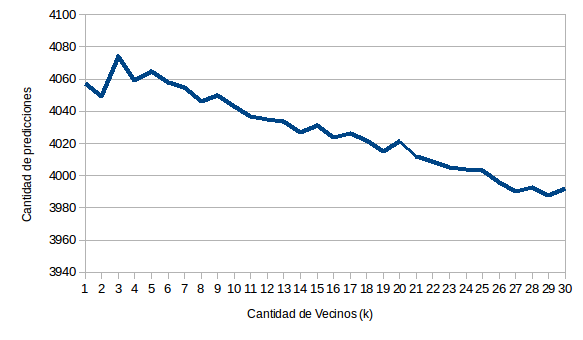
\includegraphics[scale=0.55]{nuevosResultados/knn/1.png}
\end{center}

\begin{center}
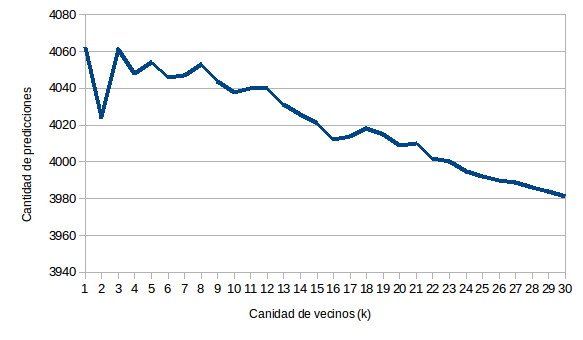
\includegraphics[scale=0.55]{nuevosResultados/knn/2.png}
\end{center}

\begin{center}
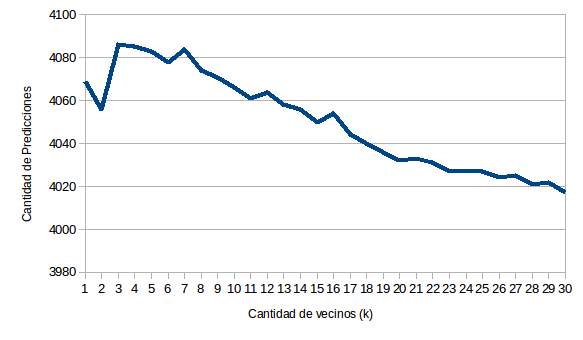
\includegraphics[scale=0.55]{nuevosResultados/knn/3.png}
\end{center}
\begin{center}
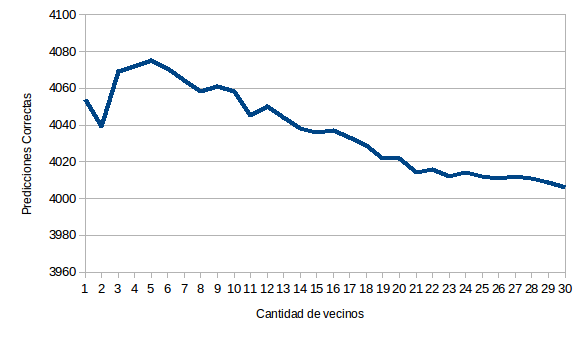
\includegraphics[scale=0.55]{nuevosResultados/knn/4.png}
\end{center}


Como se puede ver hay un patrón bastante claro en los experimentos realizados, para valores muy pequeños de $k$ los resultados son bastante buenos. Para $k=1$ se obtiene el mejor valor para $3$ de los sets que testeamos, para $k=3$ se obtiene que $4$ veces es la cantidad de vecinos que produce más aciertos, para el resto de los sets se encuentran también valores cercanos a estos. Para valores más grandes se observa un comportamiento que ratifica nuestra intuición, con un gran número de vecinos se empiezan a perder aquellos que son realmente relevantes y las predicciones empiezan a ser peores. Lo que no se esperaba era el salto en la cantidad de aciertos que vemos en los primeros valores de $k$ pero podemos entonces saber que dentro de los primeros $k$ se encuentran los mejores resultados.
\\
La distribución del mejor $k$ es la siguiente:
\begin{center}
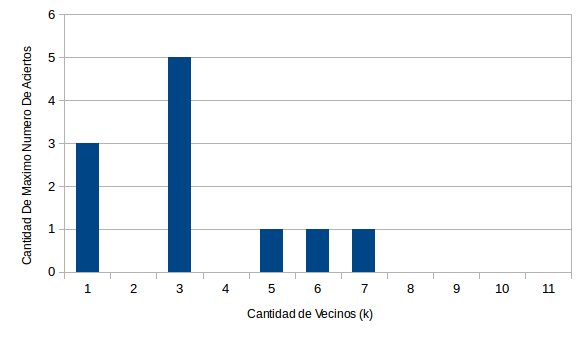
\includegraphics[scale=0.55]{nuevosResultados/knn/max.png}
\end{center}
Decidimos luego que el mejor valor para $k$ es el que produce más veces el máximo número de aciertos, es decir $k=3$. La conclusión que podemos extraer de este resultado es que para ciertos casos puede pasar que la imagen que está en primer lugar de la cola de prioridad no sea la correcta, eso pasaría para el caso en que se tiene un dígito que se parece mucho al primero de la cola, pero estos no son iguales.
Por ejemplo teniendo el dígito $x$, testeandolo con una base de datos grande en la que ningún dígito $x'$ se parece a $x$, pero teniendo otro dígito $y$ tal que se parece mucho, ese dígito $y$ va a quedar en la primera posición de la cola de resultados.
Recordemos que una vez que comparamos el dígito con toda la base de datos, se arma una cola de prioridad, ordenados semejanza entre dígitos.
Como decíamos, ese dígito $y$ puede ser considerado como un 'outlier', ya que hace que el dígito más parecido no sea el resultado correcto. Por lo tanto siempre es mejor elegir más vecinos para saber cuales dígitos aparecen en mayor cantidad y así seleccionar el de mayor cantidad de apariciones.
\\ \\
Pero, ¿Hasta qué cantidad de vecinos conviene tomar?
Si elegimos pocos vecinos podríamos tener el problema comentado anteriormente de elegir el dígito más cercano pero no el correcto.
Si elegimos muchos vecinos, lo que podría pasar es que estaríamos contando los dígitos que menos se parecen al dígito testeado, o sea, estaríamos eligiendo los peores resultados.
Según los resultados obtenidos, nos conviene elegir los primeros 3 vecinos más cercanos, ya que según los resultados testeados es el que más cantidad de aciertos obtuvo.
\\ \\
Otra observación que podemos ver de las imágenes resultantes es que para los valores $k$ pares obtenemos una menor cantidad de aciertos que para los $k$ impares.
Esto tiene sentido, ya que si tengo un dígito $x$ a testear y en la cola de prioridad obtengo como los dígitos más cercanos, por ejemplo, los dígitos $x$, $y$, $x$, $y$.
Si elegimos $k=1$ o $k=3$ el resultado sería correcto, pero si elegimos un valor $k$ par, podríamos tener un empate entre 2 dígitos y podríamos elegir el dígito incorrecto simplemente al azar, por una elección arbitraria del algoritmo, o por cualquier motivo para desempatar. Entonces por ese simple motivo, podríamos elegir mal el dígito correcto y tener menor cantidad de aciertos. En cambio, para los $k$ impares ese problema no lo tenemos y nos evitaríamos ese inconveniente, por más que después se elija el resultado correcto o no.
\\ \\
Además para estos tests realizamos una medición de tiempos para ver cómo se comportaba el algoritmo frente a un cambio en la cantidad de vecinos. Los valores promediados para cada $k$ pueden verse en el siguiente gráfico:

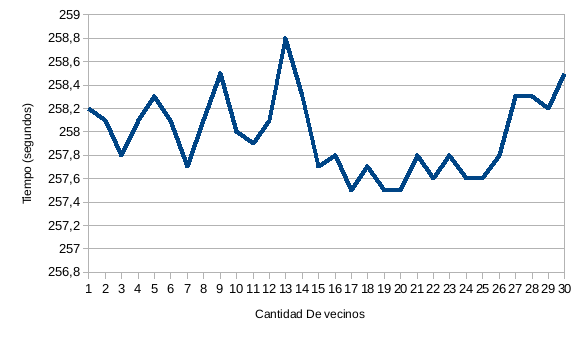
\includegraphics[scale=0.55]{nuevosResultados/knn/knntemp.png}\\

Como puede observarse, los tiempos de los algoritmos no se ven muy afectados por la variación en la cantidad de vecinos. Es muy probable que esto se deba a que el algoritmo debe comparar a la imagen que se desea comparar contra un número muy extenso de imágenes que estan en el mismo orden de magnitud.
%completar

Luego de los test decidimos que vamos a usar $k=3$ porque nos dio los mejores resultados, basado en la  cantidad de aciertos.

\subsection{PCA}
\subsubsection{Búsqueda del mejor valor de $\alpha$}
En esta sección definimos:
\begin{itemize}
	\item $\alpha$: a la cantidad de componentes principales a tomar para el $PCA$.
	\item $k$: cantidad de vecinos a considerar en el algoritmo $kNN$.
\end{itemize}
En primera instancia vamos a utilizar el método de cross-validation para intentar determinar el mejor $\alpha$ posible. Supondremos en este momento que el mejor $k$ para este caso es el encontrado en la sección anterior (aunque esto podría no ser así) y luego testeamos si esto es así o si para el $\alpha$ encontrado existe algun otro $k$ que mejora la cantidad de predicciones del sistema.
\\
Por lo tanto enfocamos nuestro análisis en obtener un valor óptimo de $\alpha$. Para este fin, partimos el conjunto de datos de entrenamiento en 10 subconjuntos y aplicamos cross-validation. Dado que este parámetro representa la cantidad de componentes principales a tener en cuenta y teniendo en mente el funcionamiento del algoritmo de $PCA$, es esperable que valores pequeños no sean beneficiosos (teniendo en cuenta que el máximo a considerar es bastante elevado), pero dado que el método de $PCA$ las ordena en base a su relevancia, se alcance un valor óptimo sin necesidad de considerarlas todas. Para esta partición de los datos de entrenamiento con 4200 imágenes para testear, tomamos $\alpha$ desde $1$ hasta $50$ y graficamos lo obtenido:

\begin{center}
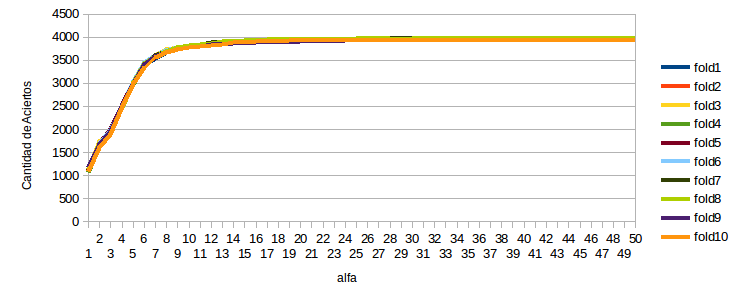
\includegraphics[scale=0.6]{nuevosResultados/pca/alfa/1.png}
\end{center}

Puede verse que para valores pequeños, aumentar en uno el $\alpha$ produce un gran aumento de aciertos. Por ejemplo, considerando el primer set para $\alpha$ igual a $1$ se obtienen $1112$ aciertos, mientras que para $\alpha$ igual a $2$ se obtienen $1680$ aciertos, esto representa un $52\%$ más de aciertos.
\\
Para valores más grandes de $\alpha$ (alrededor de $\alpha = 12$) esta tendencia empieza a estabilizarse. Por ejemplo para $\alpha = 12$ se obtienen $3845$ imágenes correctamente predecidas, pero para $\alpha = 13$ se obtienen $3869$ imágenes correctas, esto es el crecimiento de aciertos es de menos de un $1\%$.
\\
Además, para este $k-fold$ medimos los tiempos de ejecución y los promediamos para poder ver de que manera varía la ejecución de los algoritmos en función de $\alpha$:

\begin{center}
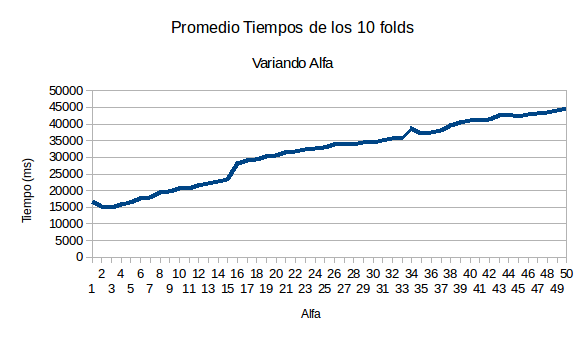
\includegraphics[scale=0.6]{nuevosResultados/pca/alfa/temp.png}
\end{center}


Cabe aclarar que estos tiempos no contemplan todo lo que se considera el 'entrenamiento' del sistema, es decir, todo el preprocesamiento que resultará en encontrar los valores principales. La justificación de esto es que el procedimiento se realizará una vez, para entrenar el sistema y luego, al momento de clasificar las nuevas imágenes este tiempo podrá ser despreciado.
\\
En este gráfico se puede ver que aumentar el $\alpha$ produce un aumento lineal de los tiempos de ejecución, de lo que se desprende que aumentar la cantidad valores principales no resulta gratuito en términos de tiempo de ejecución y tiene cierto costo asociado.
\\
Además aumentar de manera desmedida el $\alpha$ puede provocar lo que en la jerga de machine learning se denomina 'Overfitting' o Sobreajuste, que consiste en que el modelo en vez de buscar patrones sobre los cuales predecir, empieza a 'memorizar' de alguna manera los datos de entrenamiento. Esto puede conducir a que, si bien en la etapa de desarrollo se obtienen buenos niveles de predicción, cuando el modelo es puesto a prueba en algún caso real su desempeño no es el esperado\footnote{\label{note1}A Few Useful Things to Know about Machine Learning, Pedro Domingos, Department of Computer Science and Engineering, University of Washington}.
\\
Debido a todas las razones expuestas consideramos que $\alpha$ igual a $14$ será el mejor valor que podemos tomar.
\\
%falta retestear esto de abajo
\subsubsection{Búsqueda del mejor valor de $k$}

La segunda prueba a realizar es, fijando un valor de $\alpha$, analizar para que cantidad de vecinos se obtiene la mayor cantidad de aciertos.
\\
Para esto tomamos $\alpha = 14$, volvemos a dividir el conjunto de datos en $10$ sets y realizamos cross validation sobre estos, variando el $k$ desde $1$ hasta $30$.
\\
En el siguientes gráficos mostramos el resultado obtenido para los tres de los sets cuando se varía el número de vecinos:
\begin{center}
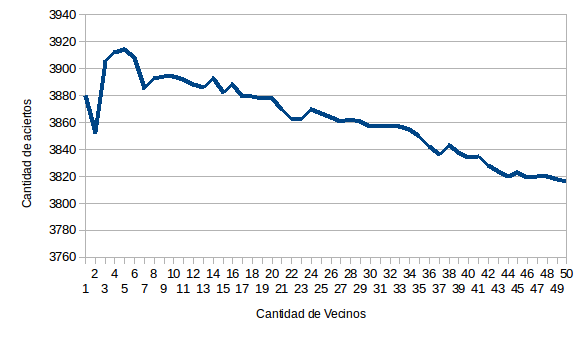
\includegraphics[scale=0.6]{nuevosResultados/pca/k/1.png}\\
\end{center}
\begin{center}
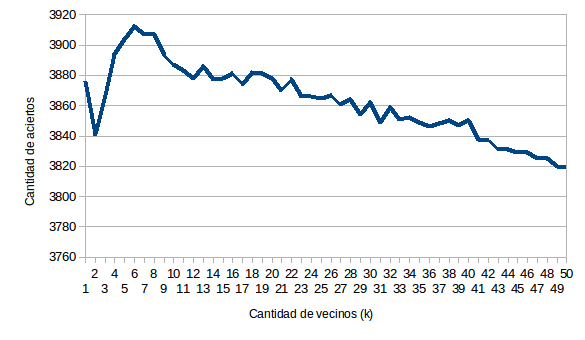
\includegraphics[scale=0.6]{nuevosResultados/pca/k/2.png}\\
\end{center}
\begin{center}
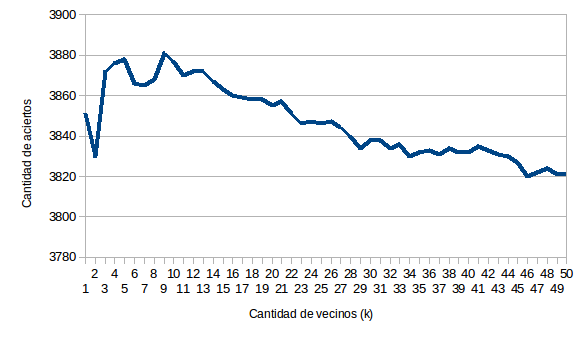
\includegraphics[scale=0.6]{nuevosResultados/pca/k/3.png}\\
\end{center}

En total, de los diez sets en tres de ellos se encontró que el número de vecinos que maximiza la cantidad de aciertos era $5$, en dos se encontró que el máximo fue $7$ y $8$, y en otros restantes el mejor fue $3$, $6$ y $9$ vecinos, cada uno.
\\
En el siguiente gráfico expresamos cómo se distribuyeron los máximos en cada conjunto del cross-validation:
\begin{center}
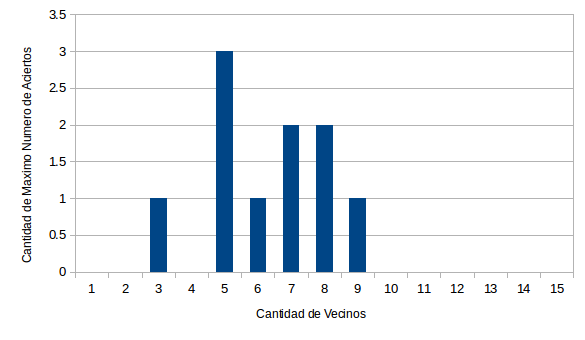
\includegraphics[scale=0.6]{nuevosResultados/pca/k/mejores.png}\\
\end{center}
De esto podemos determinar que el $k$ óptimo se encuentra en un rango entre $3$ y $9$.

Además medimos los tiempos y los promediamos para obtener una idea de cómo afectan las variaciones de $k$ a este método:
\begin{center}
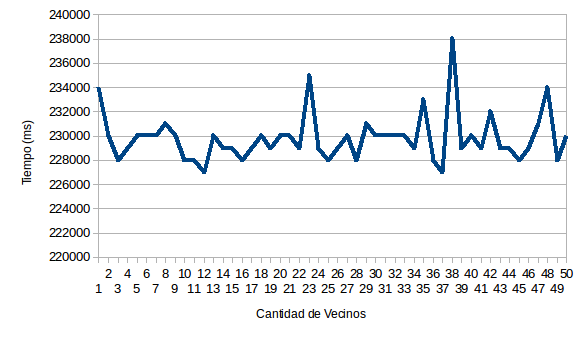
\includegraphics[scale=0.6]{nuevosResultados/pca/k/temp.png}\\
\end{center}

Como podemos ver, el número de vecinos continúa sin afectar mayormente los tiempos de ejecución incluso luego de haber reducido la dimensión de la entrada.


\pagebreak
\section{Resultados}

\subsection{An\'alisis de tiempos en funci\'on de los parametros de entrada}
En esta seccion analizaremos de manera experimental como varían los tiempos de ejecución de los algoritmos descriptos, al variar el largo y el ancho de la matriz y la cantidad de sanguijuelas del sistema.
\subsubsection{Ancho en función del tiempo}
Para comenzar, tomaremos un parabrisas con 50 sanguijuelas, tal que estas solo toquen un punto de la discretización, y para una granularidad fija de $1.0$ iremos variando el largo del parabrisas. De esta manera, comenzaremos con un parabrisas de $50 \times 50$ luego uno de $60 \times 50$ y asi aumentando de manera lineal ambos parametros hasta llegar a un parabrisas de $100 \times 50$. Resolveremos cada uno de estos sistemas utilizando ambos metodos implementados (Gauss y Descomposición LU). Los resultados obtenidos pueden verse en el siguente grafico:

\begin{center}
 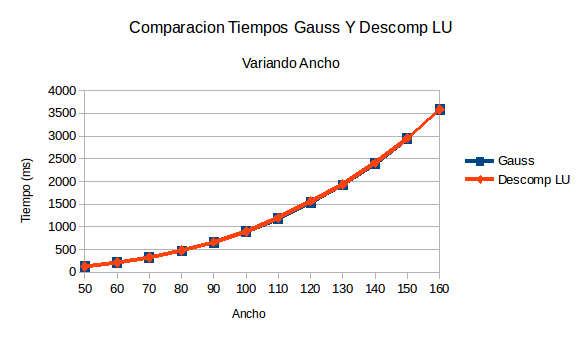
\includegraphics[width=400pt]{imagenes/testeo/anchoGauss.png}
\end{center}

Sabemos que al aumentar el largo de el parabrisas de manera lineal, aumentará de manera lineal el numero de ecuaciones en nuestra matriz de resolución. Lo que puede observarse en este grafico es que con un aumento lineal del largo del parabrisas, el tiempo de ejecución aumenta de manera cuasi-lineal. Esto era esperable ya que sabemos que tanto el gauss como la descomposición LU tienen una complejidad igual a $O(n*p^2)$, y dado que en nuestro modelado, utilizamos el largo del parabrisas para definir el tamaño de la banda en la matriz de resolución (osea $p$), era logico que al aumentar el largo, se obtuviera un aumento casi cuadratico en el tiempo de ejecución.
\\
Ahora, utilizando la misma familia de parabrisas descripta anteriormente, veremos como se comportan ambos metodos de salvación. Dado que nos aseguramos que cada sanguijuela solo toque un punto de la discretización, nos aseguramos que podremos utilizar el metodo de Sherman Morrison. Para estos algoritmos, el grafico es el siguiente:

\begin{center}
 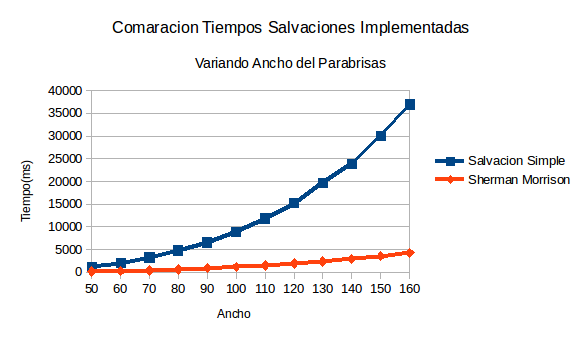
\includegraphics[width=400pt]{imagenes/testeo/anchoSalv.png}
\end{center}
%Grafico

\explicar
\subsubsection{Largo en función del tiempo}
Ahora, analizaremos que sucede dejando fijo el ancho y variando el largo del parabrisas. Las condiciones son las mismas que en el test anterior, solo que ahora el ancho permaence constante igual a $50$ y se varía el largo de $50$ a $100$.

\begin{center}
 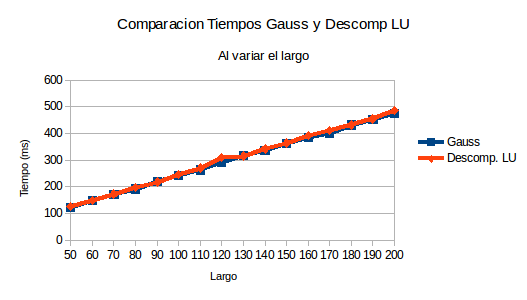
\includegraphics[width=400pt]{imagenes/testeo/largoGauss.png}
\end{center}

En este caso los tiempos de ejecución crecen de manera estrictamente lineal. Esto se debe que a diferencia del ancho, el largo no interviene en el calculo del tamaño de la banda de la matriz de resolución. Luego al aumentar el largo, solo aumenta la cantidad de incognitas $n$.
\\
Y aplicando el mismo experimento para los dos metodos de salvación:

\begin{center}
 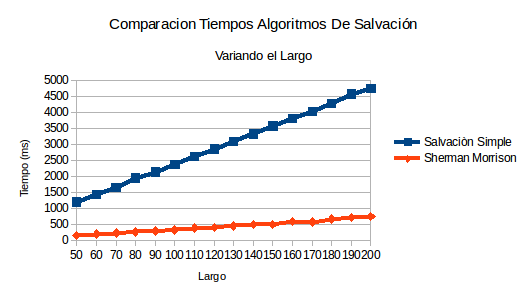
\includegraphics[width=400pt]{imagenes/testeo/largoSalv.png}
\end{center}

\explicar
\subsubsection{Cantidad de sanguijuelas en función del tiempo}
Para el siguente experimento, variaremos la cantidad de sanguijuelas y dejaremos fija tanto la granularidad como el largo y el ancho del parabrisas. Nuevamente, por una cuestión de simplicidad las sanguijuelas solo tocarán un punto de la discretización. Para el experimento tomamos un parabrisas de $100 \times 100$, una granularidad igual a $1.0$, y variamos la cantidad de sanguijuelas desde $10$ hasta $100$. Resolviendo el sistema con el algoritmo de Gauss y Descomposicion LU, se obtuvo el siguiente grafico.

\begin{center}
 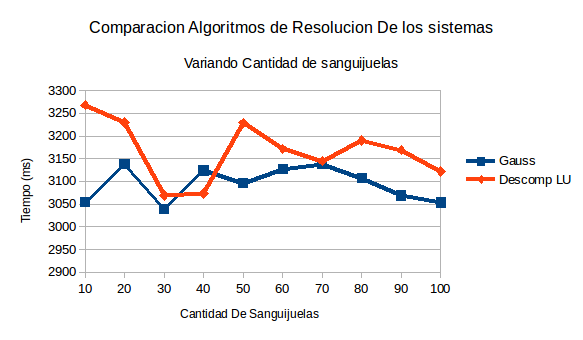
\includegraphics[width=400pt]{imagenes/testeo/sangGauss.png}
\end{center}

Como vemos, no se muestra ningun patron visible al modificar la cantidad de sanguijuelas del sistema. Esto es porque la cantidad de incognitas continua siendo la misma.
\\
Ahora utilizando el mismo experimento para el problema del ultimo disparo, resolviendo este parabrisas con ambos algoritmos, se obtuvo este grafico:

\begin{center}
 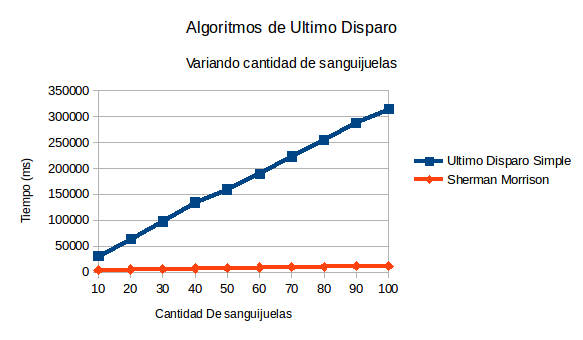
\includegraphics[width=400pt]{imagenes/testeo/sangSalv.png}
\end{center}
%Grafico
\subsubsection{Granularidad en función del tiempo}
Por ultimo, veremos como afecta variar la granularidad de la discretización para ver como se ve afectada la performance. Para este experimento se dejarán fijos el largo y el ancho, iguales a $100$, la cantidad de sanguijuelas iguales a $5$ y se variará la granularidad desde $0.4$ hasta $0.9$, aumentando de $0.1$ en cada paso. Lo obtenido es lo siguiente:

\begin{center}
 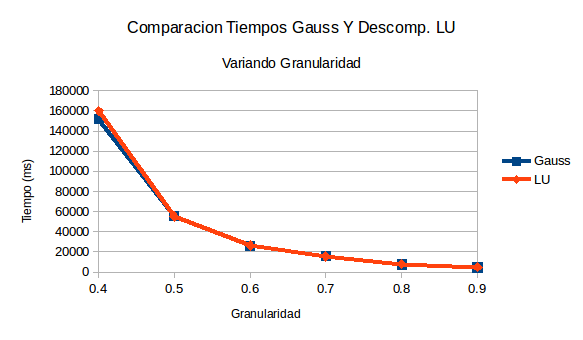
\includegraphics[width=400pt]{imagenes/testeo/granuGauss.png}
\end{center}

En el grafico puede verse que una disminucion lineal de la granularidad produce un aumento cuadratico en el tiempo de ejecución. Esto se debe a que tanto la cantidad de filas y la cantidad de columnas viene dado por el largo/ancho del paravrisas, dividido por la granularidad. Dado que el tamaño de nuestra matriz de resolución del probema viene dado por $\text{Cantidad De filas} \times \text{Cantidad De Columnas}$ esto será lo mismo que  $(\text{Largo} \times \text{Ancho}) / \text{granularidad}^2$. En esta formula puede verse claramente que disminuir la granularidad de manera lineal produce un aumento cuadratico en el numero de incognitas de nuestro problema.

\subsection{An\'alisis de temperatura y tiempos en funci\'on de las discretizaciones}
A continuaci\'on presentamos el an\'alisis y las conclusiones obtenidas de acuerdo a la experimentaci\'on realizada.
Como pudimos intuir en un primer momento, una mayor granularidad en la discretizaci\'on hace escalar r\'apidamente la cantidad de ecuaciones y variables involucradas, con lo que el tiempo de los algoritmos escala r\'apidamente. Como supusimos, ambos algoritmos (Lease, la Eliminaci\'on Gaussiana explotando la estructura banda y la factorizaci\'on LU) utilizados en el an\'alisis,  presentan diferencias de tiempo considerables, sobre todo a partir del \'ultimo caso analizado donde se termina resolviendo un sistema de ecuaciones representado en una matriz de $200 \times 200$
A continuaci\'on se presenta una lista con la granularidad utilizada y el tiempo obtenido para cada algoritmo:


\begin{table}[h]
\begin{tabular}{lll}
Granularidad & Gauss & LU \\
2 & 4.678 & 15.877 \\
1 & 41.381 & 143.102 \\
0.5 & 459.756 & 1784.492 \\
0.1 & 259967.136 & 1058285.72 \\
\end{tabular}
\end{table}



\begin{center}
 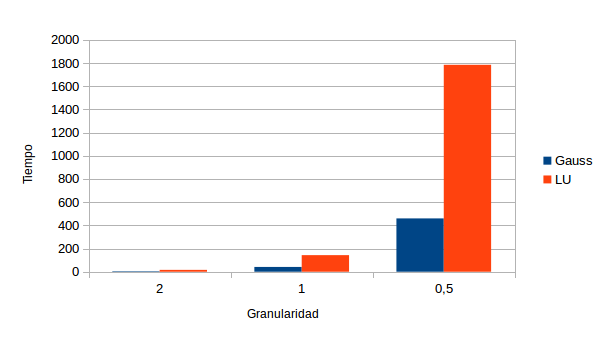
\includegraphics[width=400pt]{imagenes/grafico.png}
\end{center}


En cuanto a la distribuci\'on de calor, partiendo de la base de que un aumento en la granularidad permite una mejor representaci\'on de las sanguijuelas (son circulos), notamos que con este aumento y mejora en la representaci\'on, las temperaturas del punto cr\'itico disminuyen considerablemente. Teniendo en cuenta esta informaci\'on, queda claro como una baja granularidad impacta directamente sobre la precisi\'on de los resultados (a expensas, como vimos con anterioridad, de los tiempos de c\'omputo).
\begin{itemize}
 \item Matriz $20 \times 20$, granularidad 2.\\
  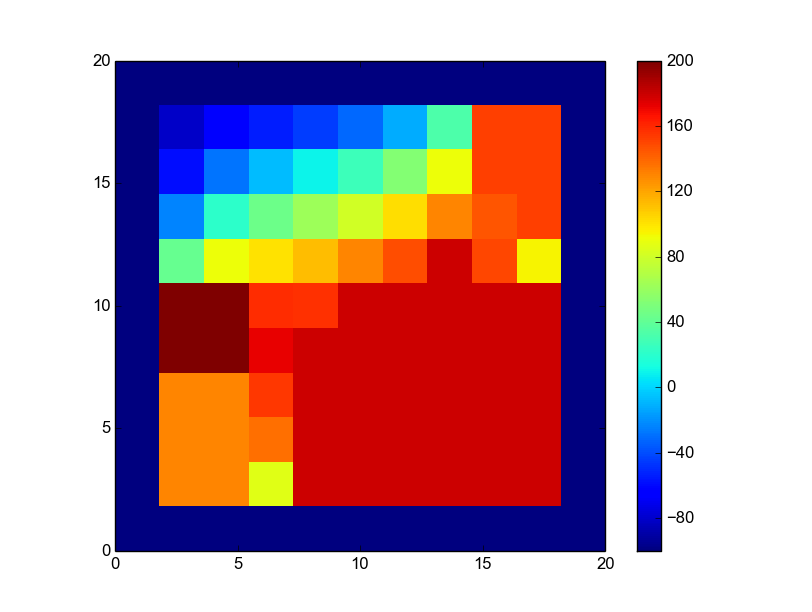
\includegraphics[width=400pt]{imagenes/imagen11.png}

 \item Matriz $20 \times 20$, granularidad 1.\\
  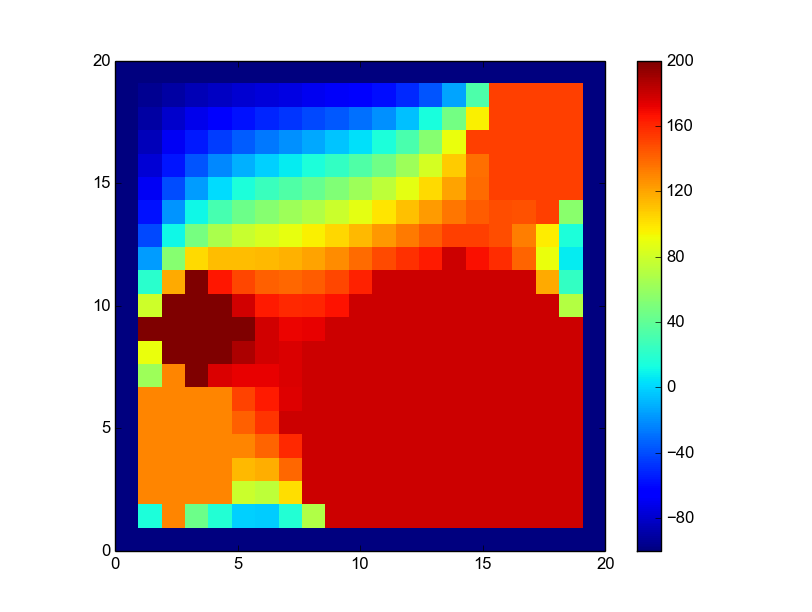
\includegraphics[width=400pt]{imagenes/imagen21.png}

 \item Matriz $20 \times 20$, granularidad 0,5.\\
  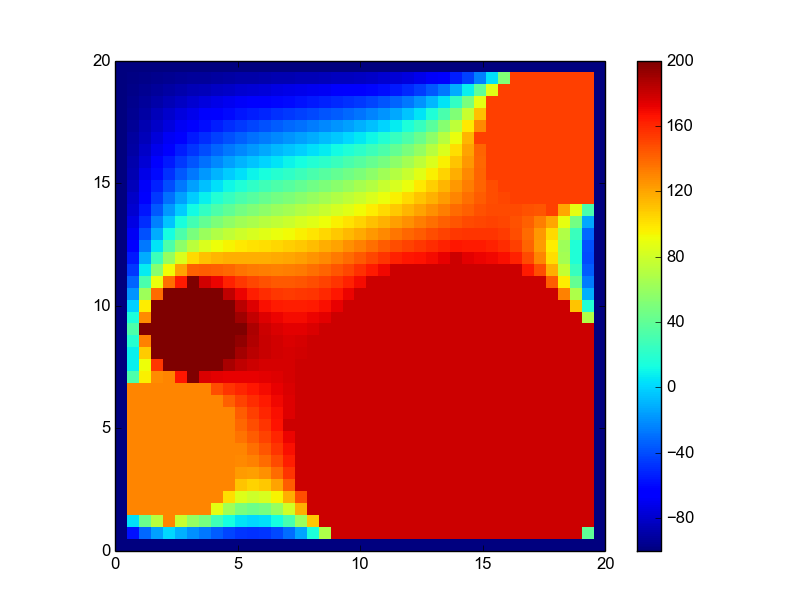
\includegraphics[width=400pt]{imagenes/imagen31.png}
  
   \item Matriz $20 \times 20$, granularidad 0,1.\\
  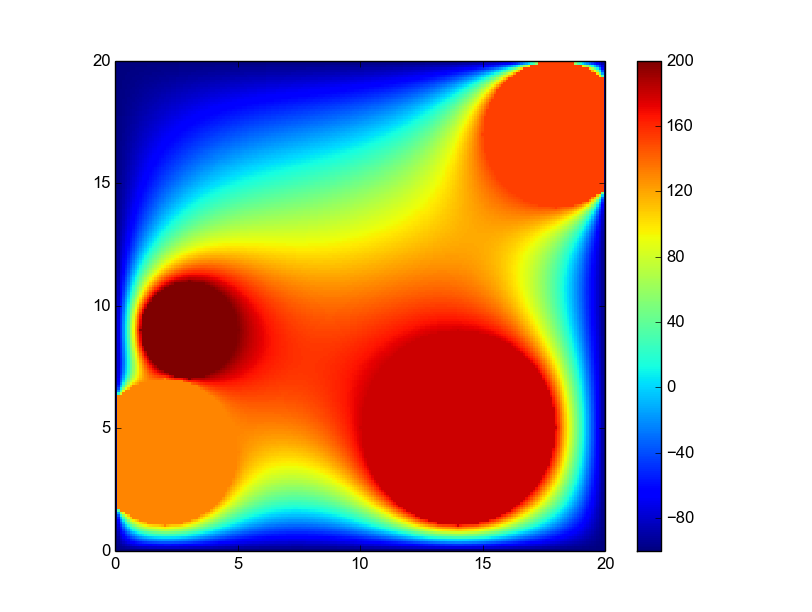
\includegraphics[width=400pt]{imagenes/imagen41.png}
\end{itemize}


Ademas se hicieron test de stress con matrices de $50 \times 50$ generadas de forma aleatoria con una misma semilla y variando la granularidad para analizar la performances de los distintos algoritmos

Algoritmo de salvacion:
\begin{center}
 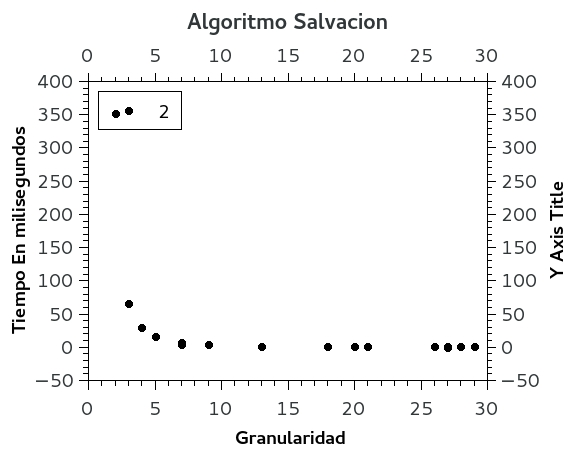
\includegraphics[width=400pt]{graficas/algoritmo salvacion.jpg}
\end{center}

Algoritmo de eliminacion gaussiana:
\begin{center}
 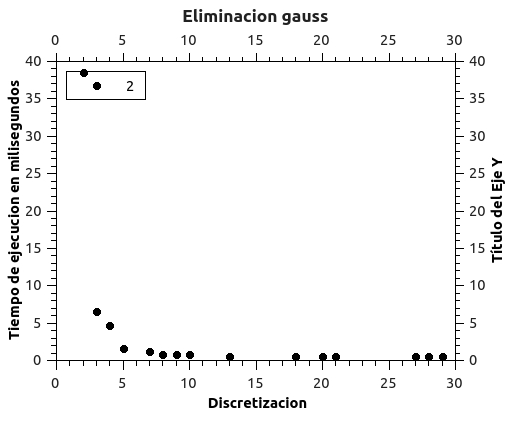
\includegraphics[width=400pt]{graficas/gauss.jpg}
\end{center}

Algoritmo de LU:
\begin{center}
 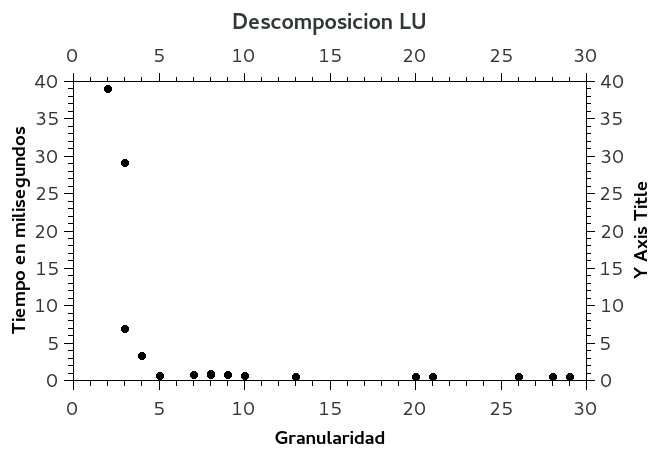
\includegraphics[width=400pt]{graficas/LU.jpg}
\end{center}

\subsection{Optimizaci\'on del c\'omputo para cambios leves del sistema}

As\'i como la particularidad de que el problema se puede plantear mediante el uso de una matriz banda permite ahorrar tiempo de c\'omputo y almacenamiento, otras especificidades del sistema o casos particulares permiten mejorar las estrategias de resoluci\'on. Para casos donde el sistema se modifica levemente, es decir que se produce un cambio en una sola fila de la matriz banda de resoluci\'on, es posible aplicar lo que se conoce como la f\'ormula de Sherman-Morrison. Lo que permite esta f\'ormula es evitar recomputar el algoritmo de eliminaci\'on gaussiana en estos casos, resumiendolo a una peque\~na cantidad de operaciones aritm\'eticas.

Para los casos donde aplica la f\'ormula de Sherman-Morrison, El c\'alculo sobre variaci\'on del sistema se realiza bajo una complejidad computacional de $O(n^2)$ mientras la resoluci\'on a trav\'es de la eliminaci\'on gaussiana cl\'asica es de $O(n^3)$, notando una mejora sustancial usando Sherman-Morrison.

Si bien notamos esta mejora te\'orica y entendemos por qu\'e sucede, no pudimos traducir esta mejora al c\'odigo. Es decir, en los resultados obtenidos no se nota una mejor\'ia respecto al caso base que es la aplicaci\'on de la Eliminaci\'on Gaussiana. Atribuimos esta diferencia entre los resultados te\'oricos y los observados a errores en el c\'odigo y/o en las mediciones ya que no se presentan otros motivos para que los tiempos se mantengan m\'as bajos utilizando Sherman-Morrison.


\pagebreak
\section{Conclusiones}

\subsection{Ventajas en el uso de una matriz banda}

Como ya discutimos en el desarollo, pudimos modelar el problema a resolver como una matriz banda. Gracias a esto es que pudimos realocar los valores en un espacio físico muy por debajo de lo que la representación matricial de un caso general requiere. Ahorrando memoria, ya que fue suficiente con almacenar los valores dentro de la banda y ahorrando tiempo de cómputo, ya que como también discutimos en la sección de desarrollo, nos limitamos a aplicar los algoritmos en la banda. De este modo obtuvimos complejidades teóricas más pequeñas que aquellas que se obtienen con el algoritmo estándar.

\subsection{Discretización de un problema continuo}

En el apartado de experimentación pudimos ver que tomando un valor de discretización muy grande, el problema que comenzó siendo continuo, pasa a ser discreto, pudiendose ver a simple vista los bloques que fueron discretizados. A medida que la discretización se vuelve mas pequeña el problema empieza a tener un comportamiento más continuo (aunque sea de manera perceptual, ya que la solución sigue siendo discreta), lo que sugiere que aumentar la discretización aumenta la presición de todo el sistema.

Sin embargo esto viene acarrea una compensación que resulta que para una discretización más pequeña, y por lo tanto exacta, el tiempo de cómputo aumenta sustancialmente. Luego a la hora de simular este problema deberá prestarse sumo cuidado a esta relación tiempo-presición dependiendo del problema en particular y el grado de confianza que se desea obtener.

\subsection{Optimizaciones Algebraicas}

Comparando ambos métodos de salvación del parabrisas pudimos ver como utilizar propiedades algebraicas y ordenar las operaciones de manera inteligente permite obtener tanto complejidades teóricas tanto como tiempos experimentales mejores. Más se noto la diferencia en los tiempos para el Sherman-Morisson ya que al realizar el producto de vectores de la manera correcta generamos menor cantidad de operaciones, acelerando el cálculo de los valores por quedarnos con un producto de vector por escalar, cambiando el orden de los productos notamos que generamos una matriz haciendo que la cantidad de operaciones se multiplique.
\\
Luego, podemos concluir que para poder resolver un problema de manera óptima es importante valerse de las propiedades específicas de las matrices con las que se trabaja, así también como la teoría del álgebra lineal.

\subsection{Otras aplicaciones}

Vemos como este tipo de problema donde el valor de cada elemento de un espacio en 2 dimensiones (o más) depende del valor de elementos cercanos puede aplicarse en diversas áreas, por ejemplo en el procesamiento de imágenes, donde el suavizado en el zoom de una imágen se puede realizar a través del promedio de los vecinos de cada pixel. También es de posible aplicación para la propagación de ondas en distintos medios. Es interesante ver también como algunas técnicas genéricas ayudan a la velocidad de cómputo y luego se pueden realizar optimizaciones dentro del dominio de cada sistema en particular, como fue en nuestro caso Sherman-Morrison para casos donde el sistema varía levemente.


\pagebreak
\section{Apendice}


\subsection{Archivos de test usados}
Dentro de la carpeta /src/testPropios se encuentran los siguientes archivos usados en la experimentacion
Archivos usados para la seccion analisis de temperatura en funcion de granularidad
\begin{itemize}
 \item sanguijuela0\_5.in
 \item sanguijuela1.in
 \item sanguijuela5.in
 \item sanguijuela10.in 
 \item test3.in
 \item test3b.in
 \item test3.in
 \item test3b.in
 \item test3.in
 \item test3b.in
\end{itemize}






\end{document}
